%!TEX ROOT=formularioMatematica.tex

\section{Progressioni}\label{sec:progressioni}
Le progressioni sono una serie di numeri in modo che tra due numeri successivi ci sia una costante
relazione. Si dividono in \textbf{aritmetiche} e \textbf{geometriche}.\\
Per gli esercizi si vada \hyperref[ex:progressioni]{qui}.

\subsection{Progressioni Aritmetiche}
Le progressioni aritmetiche hanno la caratteristica che la differenza tra due termini successivi �
sempre costante. Questa differenza si chiama \emph{ragione}.
\begin{equation*}
a_n - a_{n-1} = d \quad d = \frac{a_n-1}{n-1}
\end{equation*}
dove $d$ � la ragione e $a_n$ � un elemento qualunque di una progressione.

\subsubsection{$n$-esimo elemento}
\begin{equation*}
a_n = a_1 + d(n-1)
\end{equation*}

\subsubsection{$s$-esimo elemento riferito ad un $r$-esimo elemento}
Questa � considerabile una generalizzazione della formula precedente.
\begin{equation*}
a_s = a_r + d(s-r)
\end{equation*}

\subsubsection{Propriet� di simmetria}
\begin{equation*}
a_1+a_n = a_{k+1}+a_{n-k}\qquad\forall k
\end{equation*}

\subsubsection{Somma di una progressione}
\begin{equation*}
S_n = \frac{a_1+a_n}{2}\cdot n
\end{equation*}

\subsection{Progressioni Geometriche}
Le progressioni geometriche hanno la caratteristica che il rapporto tra due successivi elementi �
costante. Questo rapporto si chiama \emph{ragione}
\begin{equation*}
\frac{a_n}{a_{n-1}} = q \quad q:\;\begin{dcases}
q = \sqrt[n-1]{\frac{a_n}{a_1}} &\text{se concordi, per }n>2\\
q = -\sqrt[n-1]{\left\lvert\frac{a_n}{a_1}\right\rvert} &\text{se discordi}
\end{dcases}
\end{equation*}
dove $q$ � la ragione e $a_n$ � un elemento qualunque di una progressione.

\subsubsection{$n$-esimo elemento}
\begin{equation*}
a_n = a_1\cdot q^{n-1}
\end{equation*}

\subsubsection{$s$-esimo elemento riferito ad un $r$-esimo elemento}
Questa � considerabile una generalizzazione della formula precedente.
\begin{equation*}
a_s = a_s\cdot q^{s-r}
\end{equation*}

\subsubsection{Propriet� di simmetria}
\begin{equation*}
a_1\cdot a_n = a_{k-1}\cdot a_{n-k}
\end{equation*}

\subsubsection{Somma di una progressione}
\begin{equation*}
S_n = a_1\frac{1-q^n}{1-q}
\end{equation*}

\section{Calcolo combinatorio}\label{sec:calccomb}
Il calcolo combinatorio descrive i diversi modi di disporre e organizzare un finito numero di oggetti.
\\Per gli esercizi si vada \hyperref[ex:calccomb]{qui}.

\subsection{Fattoriale}
Un concetto fondamentale del calcolo combinatorio � quello di fattoriale. Esso � definito come
\begin{equation*}
n! = n\cdot (n-1) \cdot (n-2) \dotsm 2\cdot1 = \prod\limits_{1}^{n}n
\end{equation*}

\subsection{Disposizioni}
Due disposizioni si considerano distinte se almeno un elemento � diverso e non tutti devono essere 
presenti. L'ordine � importante.

\subsubsection{Semplici}
\begin{equation*}
D_{n,k} = \frac{n!}{(n-k)!} = n(n-1)\dotsm(n-k+1)
\end{equation*}

\subsubsection{Con ripetizione}
\begin{equation*}
D'_{n,k} = n^k
\end{equation*}

\subsection{Permutazioni}
Due permutazioni si considerano distine se almeno un elemento � diverso.

\subsubsection{Semplici}
\begin{equation*}
P_n = D_{n,n} = n!
\end{equation*}

\subsubsection{Con ripetizione}
\begin{equation*}
P_n^{\alpha_1,\alpha_2,\dotsc,\alpha_n} = \frac{n!}{\alpha_1!\alpha_2!\dotsm\alpha_n!}
\end{equation*}
dove $\alpha_n$ identifica il numero di ripetizioni per il relativo oggetto.

\subsection{Combinazioni}
Le combinazioni rappresentano tutti i gruppi che si possono formare da $n$ elementi considerando 
distinti due gruppi se almeno un elemento � diverso.

\subsubsection{Semplici}
\begin{equation*}
C_{n,k} = \frac{\mathscr{D}_{n,k}}{k!} = \binom{n}{k} = \frac{n!}{k!(n-k)!}
\end{equation*}

\subsubsection{Con ripetizione}
\begin{equation*}
C'_{n,k} = \binom{n+k+1}{k}
\end{equation*}

\subsubsection{Propriet� del coefficiente binomiale}
\paragraph{Simmetria}
\begin{equation*}
\binom{n}{k} = \binom{n}{n-k}
\end{equation*}

\paragraph{Per $1\leq k \leq n-1$}
\begin{equation*}
\binom{n}{k} = \binom{n-1}{k-1}+\binom{n-1}{k}
\end{equation*}

\paragraph{Per $1\leq k\leq n$}
\begin{equation*}
\binom{n}{k} = \binom{n-1}{k-1}+\binom{n-2}{k-1}+\dots+\binom{k}{k-1}+\binom{k-1}{k-1}
\end{equation*}

\paragraph{Binomio di Newton}
\begin{equation*}
(a+b)^n = \sum\limits_{k=0}^{n}\binom{n}{k}a^{n-k}b^k
\end{equation*}
da cui deriva
\begin{equation*}
2^n = \sum\limits_{k=0}^{n}\binom{n}{k}
\end{equation*}

\subsection{Schema riassuntivo}
\begin{figure}[h]
	\centering
	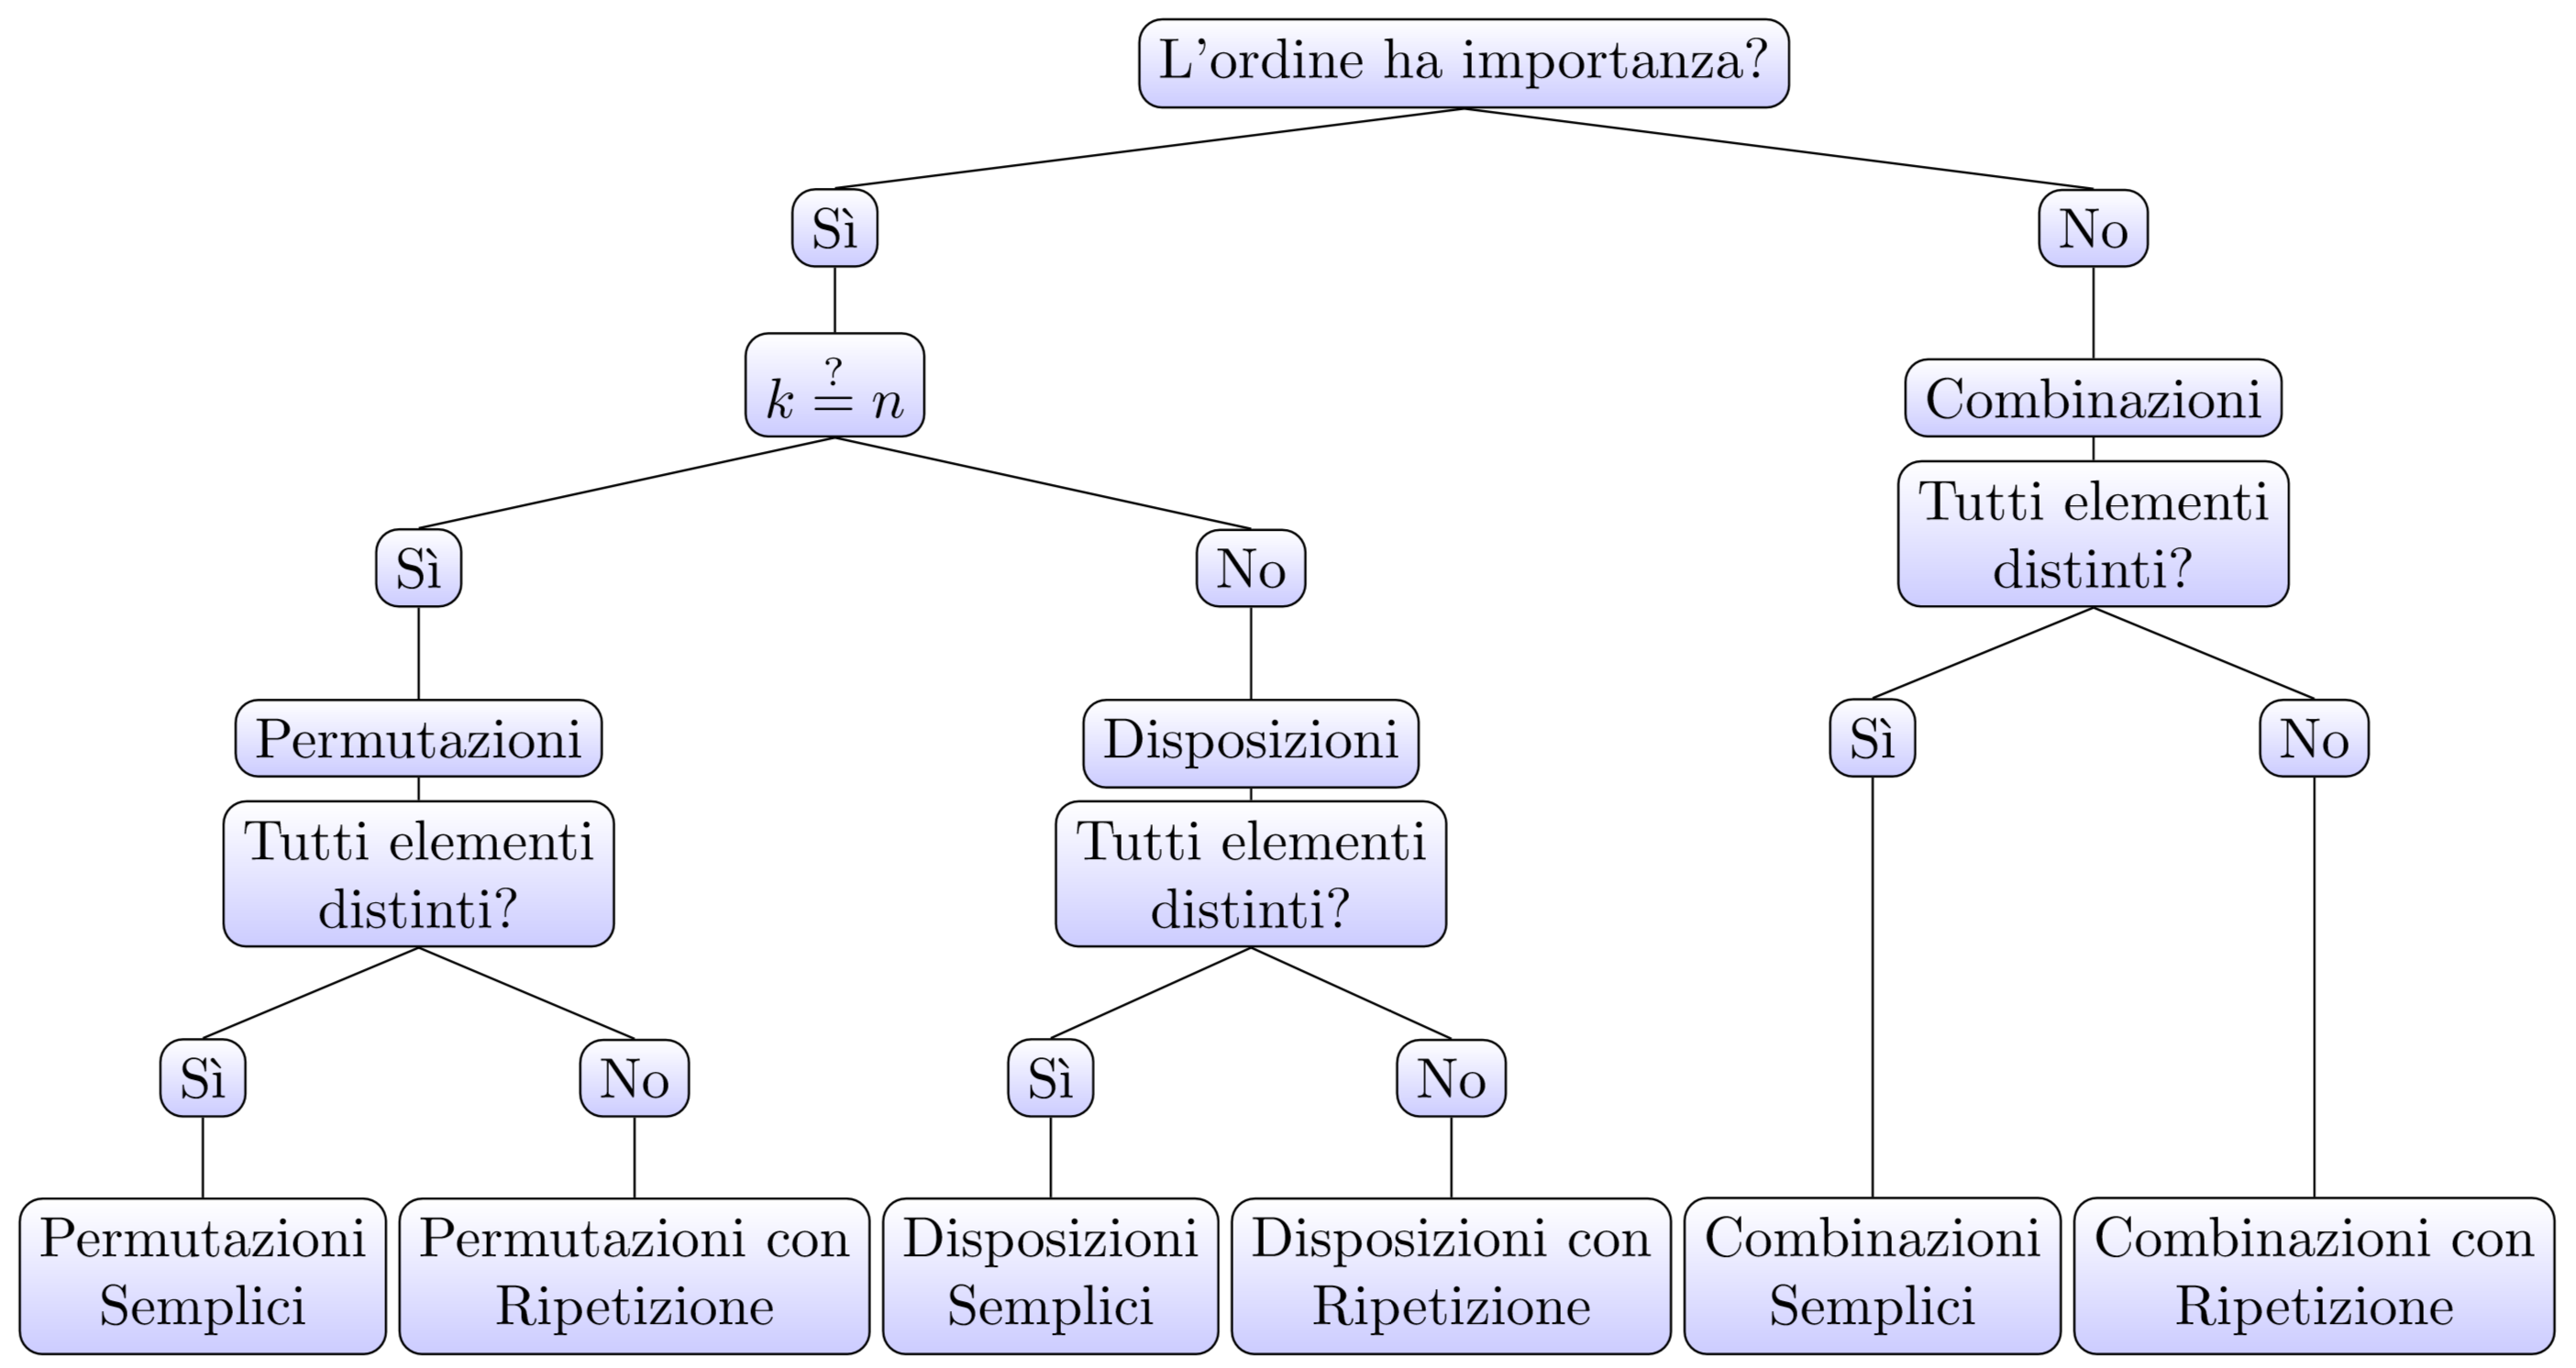
\includegraphics[width=8cm]{image/tree}
	\caption{Si risponda a ciascuna domanda per sapere che tipo di situazione il problema pone.}
\end{figure}